\newpage
\section{Symmetric abstractions}


% symmetry is cool
Symmetry is a concept from pure mathematics, which has found success in physics,
but not much else where. (why has it found such success in physics? beauty, compression, ... Occam's razor)
But what do we mean by symmetry?

% example

% formal definition
It is defined as ...

% occam's razor
Occam's razor is a core idea behind much of statistics, ML and science. Simple
hypotheses should be prefered as the are more likely to be right. This intuition
can be viewed a little more formally through a Bayesian perspective.

% symmetry and occams razor
How does symmetry relate to simplicity?

% how can symmetry help? more concretely
But, why do we care about symmetry?
\begin{displayquote}
We want the ability to identify symmetries in state-actions-rewards (/values) and use that knowledge to share rewards (/values) between 'similar' state-actions.
\end{displayquote}
It gives us a way to find 'simple' hypotheses that fit the data.
Imagine we knew that a learning problem was symmetry in some sense, for example ...
How might we explot this knowledge to learner more efficiently?
Reduce variance, generalise in more 'inteliigent' ways.

% but. discovery
But.

% relation to abstraction
???

% related work on complexity / occam's razor
This ability is currently lacking in the ML tool kit. There has been much work done
to

%  why do we care?
For sample efficiency!! Inductive bias. Generalise in the right way wthout making observations.

\subsection{Existing formalism}

\cite{Ravindran2002}

\begin{align}
P(f(s')|f(s), g_s(a)) = \sum_{s''\in [s']_f} P(s''| a, s) \\
P(f(s')|f(s), g_s(a)) = \sum_{\tilde s'\in [s']_f} \sum_{\tilde a \in [a]_{g_s}} \sum_{\tilde s \in [s]_f} P(\tilde s'| \tilde a, \tilde s) \\
\end{align}

Need to sum over all possible paths from $[s]$ to $[s']$?
Is it even possible for paths with different actions to exist?

To be done.

\begin{itemize}
\tightlist
  \item temporal symmetries
  \item approximate symmetries (algorithm and complexity)
  \item inference of symmetries under uncertainty (algorithm and complexity)
  \item complexity measure
\end{itemize}


\subsection{Exploitation}

\begin{displayquote}
\textit{Once have discovered a symmetry, how might we use it?}
\end{displayquote}

{\color{red}What simple experiments can I do!?!?!}
Could test each method of exploitation against each other. What are their advantages / disadvantages?

\subsubsection{Model minimisation}

...\cite{NARAYANAMURTHY}

\subsubsection{Output coupling}

Mahajan et al. propose to use knowledge similarity to share couple outputs.
\cite{Mahajan2017}

\begin{align*}
\chi: (S\times A) \times (S\times A) \to [0, 1] \\
\mathcal L(\theta) = \mathop{\mathbb E}_{\chi} \Big[(Q(s, a, \theta)-Q(s', a', \theta))^2 \Big]
\end{align*}

Coupling the outputs of similar state-actions. This is nice because, we might know
that $s, a$ and $s', a'$ are similar. Yet we many not have observed $s', a'$.

% Equivalent to sharing training data?!?

However, how did we know that $s, a$ and $s', a'$ are similar without seeing $s', a'$?

\subsubsection{Gradient coupling}

\begin{align*}
\nabla_{\theta} \ell(s, a, \theta) = \nabla_{\theta} \ell(s', a', \theta) \\
\chi \cdot \nabla_{\theta} \mathcal L(\theta)
\end{align*}

If $\chi$ has the structure $\chi((s, a), (s', a')) = \langle \nabla_{\theta}f(s, a, \theta), \nabla_{\theta} f(s', a', \theta) \rangle$ then will couple gradient in a certain way. NTK.

\subsubsection{Data augmentation}

Sharing targets between 'similar' inputs.
\cite{Ho2019a, Lim2019, Cubuk2018, Cubuk2019}
Discover which symmetries apply to a given domain, and at what magnitude.
The optimisation problem becomes one of picking the probability of each op and its magnitude.
There is a small set of ops (aka symmetries) that are given:
\textit{Identity, AutoContrast, Equalize, Rotate, Solarize, Color, Posterize, Contrast,
Brightness, Sharpness, ShearX, ShearY, TranslateX, TranslateY.}

Uses validation error as a reward for learning.

\subsubsection{Architecture}

Weight sharing?!? Weight coupling!?
\cite{Ravanbakhsh2017a,Abdolhosseini}
\cite{Anselmi2019}


\subsection{Comparison}

\begin{displayquote}
\textit{So which method of incorporating knowledge of symmetries is best?}
\end{displayquote}

\begin{itemize}
\tightlist
  \item Data augementation: flips.
  \item Gradient coupling: ??? gets complicated?
  \item Output coupling: regulariser on similar outputs.
  \item Architecture: mirror weights.
\end{itemize}

Equivalent?! (in this case, or in general?)
What other ways are there? Want to construct the space of possible ways to incorporate symmetries into a learner.

\subsection{Discovery}

\begin{displayquote}
\textit{How might we know that two state-action-reward (/values) are similar?}
\end{displayquote}

There are two possibilities. Because we have seen it (data / evidence / experience).
Because it follows a pattern we have observed. For example, we might have seen
that rotations of $45, 90, 135, 180$, are all similar, therefore our first guess
is that rotations of $225, 270, 315$ are also similar. (priors / inductive bias / generalisation)
{\color{red} TODO make this more readable / engaging}

[2.] Is hard. This is about generalising using an inductive bias towards symmetry.
% need a brief aside here about inductive bias and no free lunch!? no. can do it in the abstraction/discovery section

To be able to share, what do we need to know?

- That $x, y$ are similar. I.e. that $g \in G: y = g\circ x$
- Just share between all invariant datapoints?! No. This is about generalisation!!

\subsubsection{Symmetries from experience}

What does this buy us? If have sufficient data to tell us that $x$ and $y$ are
similar, say that they are mirror images of each other.
As an unsupervised pretraining step. Then apply and share labels and learn more quickly?
What else can $x$ tell us about $y$?

\cite{Yang2019}

Or end to end? As we get more certain that x and y are similar, we more strongly
encourage their symmetry through one of the methods outlined above.
Is it possible (/easier) to learn that x and y are similar (in terms of their labels) before (accurately) learning their labels.


\subsubsection{Inferring symmetries in data with priors}

Pick a simpler setting. No noise. Discrete domain. No action.
First we need to be able to identify group structures from observations of ???.
Then, we can generalise to observations of the groups action on another set.
Then, we can generalise to noisy observations.


> Ok, what data do we need to be able to infer a group structure $(Z_2, S_4, A_3, Di_8)$?

- Some vs all elements (if we need all, then isnt really an inference problem...).
<!-- (although, observing all the group elements might not be so bad, when they act on a large set!?) -->
- Pairs $c = a \circ s$ vs triples $c = a \circ ?$ (where do the triples come from?)

What information could be provided, or needs to be inferred?

- Number of elements in the group.
- The $n\times n$ relations.
- The type of group (cyclic, alternating, Sporadic) \href{https://en.wikipedia.org/wiki/Classification_of_finite_simple_groups}{ref}
- The identity of subgroups. $Z_2 \times X = \text{Obs}$

Under which constraints?

1. Identity
2. Inverse
3. Closure
4. Commutative / symmetric

***

- Impossible without triples. TODO prove.
- If we are given triples, then we have the job of matrix completion. That needs to satisfy [1,2,3,4].
- We can form triples from pairs when if we know that the transformations are linear?!
- ?

\subsubsection{Cayley completion}
% Expected to find something on the net about this. matrix completion of cayley tables. Am I thinking about it wrong?

Ok. We guessed a $n$ (or it has been given) and now we have an incomplete cayley matrix: we filled it in with some observations.

Q What is our earch space of possible cayley matrices? How large is it?
How does a new piece of data reduce the number of possible cayley tables?

\subsubsection{How easy is it to solve this inference problem?}

Want to have an inductive bias towards simpler symmetries. But, how can we do this without needing to represent all possible symmetries?


\subsubsection{Generalisation to ???}

If we can solve: infer group structure from missing data.
Then we can solve:

\subsubsection{Notes}

- What about symmetries that are products of subgroups? $S = Z_2 \times Z_3$?
Are they easier to infer?
- Within the same $n$. Is there a notion of more or less complex group structures??
- Need to show that NNs dont have the right symmetric inductive bias. They dont generalise.

Examples

- Knowing that; range $= [0,360)$, and $0, 45, 90, 135, 180$, all are similar. I quess that we are in cyclic group $8$ and therefore $225, 270, 315$ are also similar. Key is that I know that $0, 45, 90, 135, 180$ are related by $0+0, 0+45, 0+45+45, 0+45+45+45, 0+45+45+45+45$.
- Cart pole. $V^{\pi(s, a)}(s') = V^{\pi(-s, -a)}(-s') \forall s'$.



\subsubsection{Complexity}

Uniqueness, ...?

How hard is it to find symmetries?
First, what do we mean by a symmetry?

\begin{align}
x, y \in X : \exists G \cdot x \cap
\end{align}




\subsection{n-dimensional Cart pole}

\begin{displayquote}
  \textit{How can we test a learners ability to detect symmetries and exploit them?}
\end{displayquote}

We propose a simple test, the n-dimensional cart pole: a generalisation of the
cart pole problem to $n$ dimensions. Rather than receiving observations in
$\mathbb{R}^4$ (the position, velocity, angle and angular velocity), observations are
in $\mathbb{R}^{4\times n}$. And the action space is generalised from $\{0,1\}$ (left and right),
to $\{0,1\}^{n}$.

\cite{Brockman2016,baselines}

% What makes this problem hard??

% Existing envs dont test this because!?!?

\subsubsection{How is this problem symmetric?}

Well, the original cart pole problem has a few symmetries in it. But these are
not central to the ...

Many people realise that this problem can be reduce to $n$, one dimensional cart pole problems.
But the learner needs to infer that.

More formally. How does this problem have symmetry?
Permutations of the observation-action space perserve the problem.

\subsubsection{How might a learner exploit this knowledge to learn more effiicently?}

What advantage is provided by this knowledge?

If we knew that the problem can be decomposed into $n$ identical subproblems,
then that means we are gathering $n$ times the data for each subproblem.
So, we should see a factor of $n$ speed up in learning.

This is the same argument made here [quotient groups appendix...].

For a learner that doesnt know of the symmetries. How is this problem hard?
The more dimensions there are, the more ways there are to fail.
Consider how exploration is done. In a single dimension, a greedy action is
taken with some chance of explorating instead.

Maybe you correctly balanced the pole in all dimensions except one. To bad, you dont get any reward.



\subsection{Experiments}

What about if we rotate the observations. So the obervations are not aligned with the actions?
Or generalising to n+1? Could start the agent off with n+1 dims. But set them to observe nothing / actions do nothing. Until t > T?

\begin{figure}
  \centering
  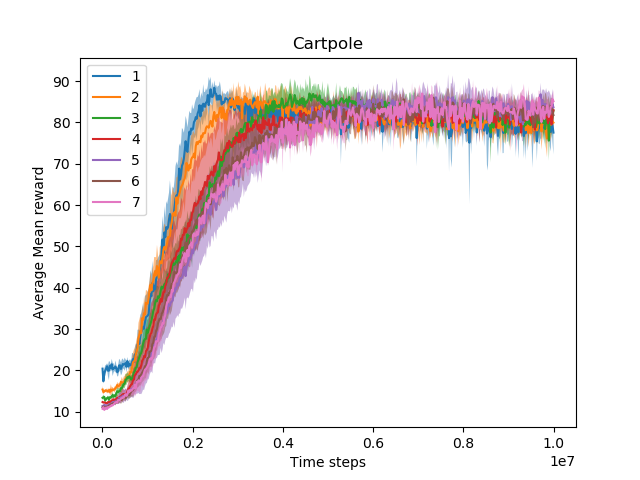
\includegraphics[width=1\textwidth,height=0.5\textheight]{../../pictures/figures/multibinary-nd-cart.png}
  \caption{PPO2 solving the nd cartpole problem with access to a \textit{MultiBinary} action space that grows with $N$.}
\end{figure}

\begin{figure}
\centering
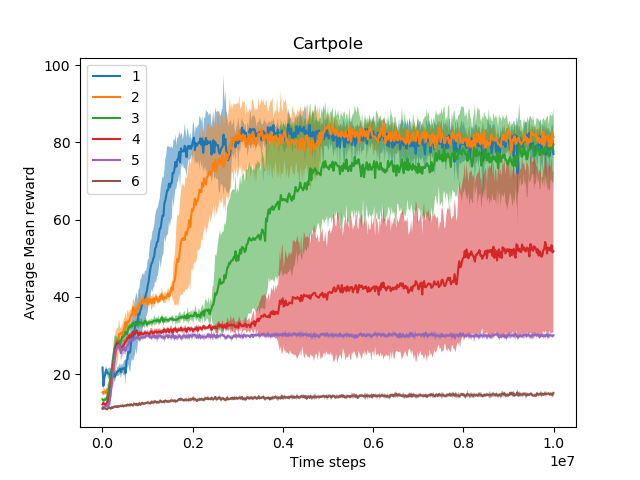
\includegraphics[width=1\textwidth,height=0.5\textheight]{../../pictures/figures/discrete-nd-cart.png}
\caption{PPO2 solving the nd cartpole problem with access to a \textit{Discrete} action space that grows with $2^N$.}
\end{figure}


\textit{Note: Average mean reward refers to the fact that we have averaged (n=5)
the mean reward (per episode). Also, this reward is the training performance.
Generalisation in RL can mean a few things.}

It seems surprising that access to the \textit{MultiBinary} action space provides such an advantage.
Also, it seems surprising that the an increase of 6 dimensions only results in approximately a ~2 million increase in the data required.
Is the learner doing some sort of intelligent sharing?
Why is it so hard for the Discrete learner? What operation does it find hard to learn. The ability to decode? $n$ bits to $2^n$ onehots?

Also, interesting to note that the 1D learner equipped with a \textit{Discrete}
action space achieves max performance at ~1.75 million samples, while the learner
equipped with a \textit{MultiBinary} action space achieves max performance at ~2.25 million samples. (significant??)

\subsection{No free lunches}

We want to


\subsection{Related work}

Relationship to disentanglement. \cite{Higgins2018} which makes a lot of sense because ...

Connection to causal heirarchy. Cite Pearl. Association, intervention, counterfactuals.
Also recently noted by \cite{Caselles-Dupre2019}, ... where they assume that
the group actions are the actions of the RL environment.
This doesnt really make sense. Also, will miss many symmetries like ???

A couple parts. Discovery of symmetries, explotation of the knowledge of symmetries.

Unsuperivsed dicovery. Not much success yet. Only when using some kind of supervised signal.


From the right perspective, it can be seen that there are many existing ideas in
 ML that exploit the knowledge of symmetries.

- Data augmentation (The D2 group (ref) for images, flips, rotations.)
- Data sharing (aka duplicate tuples \cite{Ho2019a})
- Gradient coupling (aka auxiliary loss \cite{Ho2019a})
- Weight sharing \cite{Ravanbakhsh2017a}

We discuss these equivalences in appendex [].



Exploitation. Data augmentation, ...?


\subsection{Future work}

Formalise what we mean by 'simple'. Occam's razor. Compression, symmetry.

AutoAugment. Finding symmetries?!
\cite{Ho2019a}

\subsection{Characterising symmetries for RL}

Symmetries can be uniquely characterised by their invariants \cite{PeterOlver1999}.
What are the interesting invariants of MDPs? And how do they ???

- We have n different 'symmetries'. But are they really different?
- Which symmetries share some invariants?
-
